\chapter{Mixed action setup}%\addcontentsline{toc}{chapter}{Mixed action setup}

%%%%%%%%%%%%%%%%%%%%%%%%%%%%%%%%%%%%%%%%%%%%%%%%%%%%%%%%%%%
%%%%%%%%%%%%%%%%%%%%%%%%%%%%%%%%%%%%%%%%%%%%%%%%%%%%%%%%%%%
%%%%%%%%%%%%%%%%%%%%%%%%%%%%%%%%%%%%%%%%%%%%%%%%%%%%%%%%%%%
%%%%%%%%%%%%%%%%%%%%%%%%%%%%%%%%%%%%%%%%%%%%%%%%%%%%%%%%%%%

\label{ch_ma}

%%%%%%%%%%%%%%%%%%%%%%%%%%%%%%%%%%%%%%%%%%%%%%%%%%%%%%%%%%%
%%%%%%%%%%%%%%%%%%%%%%%%%%%%%%%%%%%%%%%%%%%%%%%%%%%%%%%%%%%
%%%%%%%%%%%%%%%%%%%%%%%%%%%%%%%%%%%%%%%%%%%%%%%%%%%%%%%%%%%
%%%%%%%%%%%%%%%%%%%%%%%%%%%%%%%%%%%%%%%%%%%%%%%%%%%%%%%%%%%

\section{Motivation}
\label{ch_ma:sec:introduction}

The lattice setup used in this thesis is based on a mixed action with Wilson $\mathcal{O}(a)$ improved quarks (see Sec.~\ref{ch_foundation:subsec:Wilson}) in the sea and fully twisted Wilson tm quarks (see Sec.~\ref{ch_foundation:subsec:tm}) in the valence, whose goal is to control cutoff effects in the context of studies of flavor physics in the charm sector. These effects are of order $\mathcal{O}(am_c)$ with $m_c$ the mass of the charm quark. The use of Wilson tm fermions at maximal twist allows to remove such $\mathcal{O}(am_c)$ lattice artifacts without the need of computing specific improvement coefficients proportional to the charm quark mass, thus providing an alternative way to control the continuum limit extrapolations. Furthermore, the mixed action is yet another valid lattice regularization which provides an independent way of measuring physical observables on the lattice. In this respect, it will allow us to quote independent results for the gradient flow scale $t_0$ (see Sec.~\ref{ch_ss}), the charm quark mass and the $D_{(s)}$ mesons decay constants~\citep{charm} (see Sec.~\ref{ch_charm}). In the future, we also plan to extend this setup to the determination of the light and strange quark masses.

For the definition of the mixed action approach, we recall eq.~(\ref{ch_foundation:eq:path_int})
\begin{align}
\left<O^{ij}(x_1)O^{ji}(x_2)\right>&=-\frac{1}{\mathcal{Z}}\int\mathcal{D}[U]e^{-S_{\textrm{G}}[U]-S_{\textrm{eff}}[U]} \notag \\
&\times{\textrm{tr}}\left(\Gamma D_i^{-1}(x_1,x_2)\Gamma D_j^{-1}(x_2,x_1)\right),\\
S_{\textrm{eff}}[U]&=-\sum_i^{N_f}\textrm{log det}(D_i).
\end{align} 
We see that the Dirac operator $D$ appears first in the Boltzmann factor $e^{-S_{\textrm{G}}[U]-S_{\textrm{eff}}[U]}$, which characterizes the fields of the sea sector, with which the set of gauge ensembles is generated (see Appendix~\ref{appex_simulations}), and then in the fermionic observable whose expectation value we are interested in, depending on fields of the  valence sector. The calculation is thus divided in two separate stages of the analysis: the first one corresponds to the generation of gauge ensembles, and the other to the inversion of the Dirac operator on those gauge configurations (see Appendix~\ref{appex_solvers}). This procedure in principle allows for the use of different regularizations of the Dirac operator in these two steps or sectors of the theory. In general, a mixed action approach can introduce unitarity violations even once the continuum limit is taken, unless the physical quark masses in both sea and valence coincide. This means that our setup will require a tuning procedure in which the values of the Wilson twisted mass parameters are chosen such that the physical values of quark masses in the valence sector are matched to the corresponding ones in the sea sector.

The flavor content of our setup is as follows: on the one hand, the sea sector has $N_f=2+1$ flavors, i.e. two mass-degenerate light quarks (corresponding to the $u$ and $d$ flavors) with mass $m_l$ and one strange quark with mass $m_s$. On the other hand, the valence sector consists of $N_f=2+1+1$ flavors, thus adding a charm quark. Since we have $N_f=2+1$ in the sea and $N_f=2+1+1$ in the valence, the flavors we need to match are those of the light and strange quarks, treating the charm quark in the valence as a partially quenched flavor. 

In order to perform the matching of the theory, we need to know beforehand the value of the quark masses in the sea sector. This means that we need lattice measurements in the fully unitary Wilson fermions setup (using the Wilson regularization in the sea and valence) in addition to the mixed action regularization. We therefore consider two sets of data: those coming from the Wilson unitary setup, which we refer to as sea or Wilson results, and those coming from the mixed action itself. The use of these two sets of data will further improve the control of the scale setting analysis, as we will see in Sec.~\ref{ch_ss}. In addition to the matching of the sea and valence sectors, we also need to tune the valence action parameters to enforce full twist and automatic $\mathcal{O}(a)$ improvement.

The Chapter is structured as follows. In Sec.~\ref{ch_ma:sec:Sea} we discuss the sea sector details: ensembles under study, lattice actions and boundary conditions. In Sec.~\ref{ch_ma:sec:Valence} we discuss the valence sector, which employs Wilson tm quarks. In Sec.~\ref{ch_ma:sec:chiral_traj} we discuss the line of constant physics along which the ensembles under study were generated. They follow a chiral trajectory towards the physical point that suffers small mistunings and that must be corrected by performing small mass corrections. We discuss the details of a mass shifting procedure to account for these effects. Finally, in Sec.~\ref{ch_ma:sec:matching} we deal with the matching of sea and valence sectors though pseudoscalar masses in order to impose equal physical quark masses in both sectors and to recover unitarity in the continuum. We also explain the procedure to tune Wilson tm valence quarks to maximal twist.

%%%%%%%%%%%%%%%%%%%%%%%%%%%%%%%%%%%%%%%%%%%%%%%%%%%%%%%%%%%
%%%%%%%%%%%%%%%%%%%%%%%%%%%%%%%%%%%%%%%%%%%%%%%%%%%%%%%%%%%
%%%%%%%%%%%%%%%%%%%%%%%%%%%%%%%%%%%%%%%%%%%%%%%%%%%%%%%%%%%
%%%%%%%%%%%%%%%%%%%%%%%%%%%%%%%%%%%%%%%%%%%%%%%%%%%%%%%%%%%

\section{Sea sector}
\label{ch_ma:sec:Sea}

The gauge ensembles that we employ are CLS ensembles~\citep{Bruno:2014jqa,Mohler:2017wnb} with $N_f=2+1$ non-perturbatively $\mathcal{O}(a)$ improved Wilson fermionsn (see eq.~(\ref{ch_foundation:eq:DW_impr})). They use the Lüscher-Weisz gauge action~\citep{Luscher:1985zq} defined in eqs.~(\ref{ch_foundation:eq:SG_impr}-\ref{ch_foundation:eq:LW}) which, following the Symanzik improvement program, is  tree-level improved at $\mathcal{O}(a^2)$.

For most of the ensembles, open boundary conditions (OBC) in time are
used for the gauge fields, since it has been observed that the use of
periodic boundary conditions (PBC) leads to a steep dependence in the
scaling of  the autocorrelation times as one approaches the continuum
limit, a problem known as critical slowing down. This is related to
the existence of topologically disconnected sectors in gauge field
space, which prevents the algorithm to sample correctly different
topological sectors. In contrast to this, OBC let the topological
charge flow through the boundaries and thus avoids the problem of
topology freezing as one approaches the continuum. All ensembles use PBC in the spatial directions.

The ensembles we consider have 5 different values of the lattice spacing, and for each of them there is one ensemble at the symmetric point, which is defined as $m_l=m_s$, or equivalently for the hopping parameter $\kappa$ (see eq.~(\ref{ch_foundation:eq:kappa})) as $\kappa_l=\kappa_s$. As we will see, all the ensembles, reported in Table~\ref{apex_ensembles:tab:ens}, follow the chiral trajectory defined in eq.~(\ref{ch_ma:eq:chiral_traj}) below.


%%%%%%%%%%%%%%%%%%%%%%%%%%%%%%%%%%%%%%%%%%%%%%%%%%%%%%%%%%%
%%%%%%%%%%%%%%%%%%%%%%%%%%%%%%%%%%%%%%%%%%%%%%%%%%%%%%%%%%%
%%%%%%%%%%%%%%%%%%%%%%%%%%%%%%%%%%%%%%%%%%%%%%%%%%%%%%%%%%%
%%%%%%%%%%%%%%%%%%%%%%%%%%%%%%%%%%%%%%%%%%%%%%%%%%%%%%%%%%%


\section{Valence sector}
\label{ch_ma:sec:Valence}

In the valence sector, we employ an $N_f=2+1+1$ fully-twisted Wilson tm fermion action (see Sec.~\ref{ch_foundation:subsec:tm}), whose Dirac operator reads
\begin{equation}
D_{\textrm{W}}+\boldsymbol{m}^{\textrm{(v)}}+i\boldsymbol{\mu}^{\textrm{(v)}}\gamma_5,
\end{equation}
with 
\begin{gather}
\boldsymbol{\mu}^{\textrm{(v)}}={\textrm{diag}}(\mu_l,-\mu_l,-\mu_s,\mu_c)^{\textrm{(v)}}, \quad
\boldsymbol{m}^{\textrm{(v)}}={\textrm{diag}}(m_l,m_l,m_s,m_c)^{\textrm{(v)}}.
\end{gather}
In particular, we use the same standard quark mass for all flavors $m_l^{\textrm{(v)}}=m_s^{\textrm{(v)}}=m_c^{\textrm{(v)}}\equiv m^{\textrm{(v)}}$.

As discussed in Sec.~\ref{ch_foundation:subsec:tm}, imposing full twist means that the twist angles $\alpha_i$ fulfill
\begin{equation}
{\textrm{cot}}\;\alpha_i=\frac{m_i^{\textrm{R}}}{\mu_i^{\textrm{R}}}=0.
\end{equation}
To do so, it is enough to impose that the PCAC quark masses in eq.~(\ref{ch_observables:eq:PCAC}) vanish in the light-quark sector. When this is the case, automatic $\mathcal{O}(a)$ improvement of valence observables is obtained, up to $\mathcal{O}(a\textrm{tr}\left(M_q\right))$ cutoff effects due to the sea-quark masses. However, these effects are expected to appear at $\mathcal{O}(g_0^4)$ in perturbation theory.

In order to set the valence parameters for which sea and valence physical quark masses are matched  while simultaneously ensuring that the maximal twist condition is met, we employ a grid of valence parameter values $\left(\kappa,\mu_l,\mu_s\right)^{\textrm{(v)}}$ around an estimate of the target point in order to perform small interpolations that allow us to reach the target point $\left(\kappa,\mu_l,\mu_s\right)^{\textrm{(v)*}}$.

%%%%%%%%%%%%%%%%%%%%%%%%%%%%%%%%%%%%%%%%%%%%%%%%%%%%%%%%%%%
%%%%%%%%%%%%%%%%%%%%%%%%%%%%%%%%%%%%%%%%%%%%%%%%%%%%%%%%%%%
%%%%%%%%%%%%%%%%%%%%%%%%%%%%%%%%%%%%%%%%%%%%%%%%%%%%%%%%%%%
%%%%%%%%%%%%%%%%%%%%%%%%%%%%%%%%%%%%%%%%%%%%%%%%%%%%%%%%%%%

\section{Chiral trajectory}
\label{ch_ma:sec:chiral_traj}

The set of CLS ensembles that we use are generated along the trajectory in the quark mass plane defined by a constant trace of the bare sea ``(s)'' quark mass matrix
\begin{equation}
\label{ch_ma:eq:chiral_traj}
{\textrm{tr}}\left(M_q^{\textrm{(s)}}\right)=2m_{l}^{\textrm{(s)}}+m_{s}^{\textrm{(s)}}={\textrm{cnst}}.
\end{equation}
This trajectory ensures that at a given value of the lattice spacing, the improved bare coupling 
\begin{equation}
\tilde{g}_0^2=g_0^2\left(1+ab_g{\textrm{tr}}\left(M_q^{\textrm{(s)}}\right)\right),
\end{equation}
remains constant as we vary the sea-quark masses to approach the physical point. Note that for the Wilson unitary setup, sea and valence quark masses are the same, but not for the mixed action setup. To ensure that this trajectory crosses the physical point, we define the dimensionless quantities
\begin{align}
\label{ch_ma:eq:phi2}
\phi_2&=8t_0m_{\pi}^2,\\
\label{ch_ma:eq:phi4}
\phi_4&=8t_0\left(m_K^2+\frac{1}{2}m_{\pi}^2\right),
\end{align}
which at leading order (LO) in ChPT are proportional to the renormalized quark masses
\begin{align}
\phi_2&\propto m_l^{\textrm{R}},\\
\phi_4&\propto2m_l^{\textrm{R}}+m_s^{\textrm{R}}={\textrm{tr}}\left(M_q^{\textrm{R}}\right).
\end{align}
The trace of the renormalized quark mass matrix ${\textrm{tr}}\left(M_q^{\textrm{R}}\right)$ is in turn proportional to the bare quark mass matrix up to $\mathcal{O}(a)$ cutoff effects
\begin{equation}
{\textrm{tr}}\left(M_q^{\textrm{R}}\right)=Z_mr_m\left[\left(1+a\bar{d}_m{\textrm{tr}}\left(M_q\right)\right){\textrm{tr}}\left(M_q\right)+ad_m{\textrm{tr}}\left(M_q^2\right)\right].
\end{equation}
By setting the sea value of $\phi_4$ to its physical value for all ensembles one thus imposes that the trace of the renormalized quark mass matrix is constant up to residual lattice artifacts and higher order effects in ChPT.

To correct for these mistunings, we perform small mass shifts~\citep{Bruno:2016plf} in the bare sea-quark masses by Taylor expanding lattice observables at first order as follows
\begin{equation}
\label{ch_ma:eq:mass_shift}
{O}\left(m_l^{\textrm{(s)'}},m_s^{\textrm{(s)'}}\right)={O}\left(m_l^{\textrm{(s)}},m_s^{\textrm{(s)}}\right)+\sum_q\left(m_q^{\textrm{(s)'}}-m_q^{\textrm{(s)}}\right)\frac{d{O}}{dm_q^{\textrm{(s)}}},
\end{equation}
with the total derivative given by
\begin{equation}
\label{ch_ma:eq:md}
\frac{d{O}}{dm_q^{\textrm{(s)}}}=\sum_i\frac{\partial{O}}{\partial \left<P_i\right>}\left[\left<\frac{\partial P_i}{\partial m_q^{\textrm{(s)}}}\right>-\left<P_i\frac{\partial S}{\partial m_q^{\textrm{(s)}}}\right>+\left<P_i\right>\left<\frac{\partial S}{\partial m_q^{\textrm{(s)}}}\right>\right].
\end{equation}
Here $O=O\left(\left<P_i\right>\right)$ is an arbitrary lattice observable and $\{P_i\}_{i=1,2,...}$ is the set of primary observables on which it depends, in our case the corresponding mesonic two-point functions and the gradient flow action density. The first term within the square brackets in the right-hand side of this equation corresponds to the valence contribution to the derivative, while the two subsequent terms involving the action $S$ correspond to the sea contributions. Note that for the Wilson unitary setup, all terms contribute in fermionic observables, while for the mixed action setup, since the two-point functions $\{P_i\}$ do not depend explicitly on $m_q^{\textrm{(s)}}$, the first term in the right-hand side of eq.~(\ref{ch_ma:eq:md}) vanishes in fermionic observables. For the gradient flow scale $t_0$, only the terms involving the action $S$ in eq.~(\ref{ch_ma:eq:md}) contribute.

In particular, the sum over $q$ in eq.~(\ref{ch_ma:eq:mass_shift}) can be done in any direction of the quark mass plane, and following~\citep{Strassberger:2021tsu} we choose to mass shift only the strange quark. For practical purposes, since for each ensemble we mass shift all relevant observables to the physical value of $\phi_4$ in the sea sector $\phi_4^{\textrm{(s)}}=\phi_4^{\textrm{ph}}={\textrm{const.}}$, following~\citep{Strassberger:2023xnj} we rewrite the Taylor expansion at first order as
\begin{equation}
{O}\left(\phi_4^{\textrm{(s)'}}=\phi_4^{\textrm{ph}}\right)={O}\left(\phi_4^{\textrm{(s)}}\right)+\left(\phi_4^{\textrm{ph}}-\phi_4^{\textrm{(s)}}\right)\frac{d{O}}{d\phi_4^{\textrm{(s)}}},
\end{equation}
with
\begin{equation}
\label{ch_ma:eq:dOdphi4}
\frac{d{O}}{d\phi_4^{\textrm{(s)}}}=\frac{d{O}/dm_s^{\textrm{(s)}}}{d\phi_4^{\textrm{(s)}}/dm_s^{\textrm{(s)}}}.
\end{equation}
Note that the sea value $\phi_4^{\textrm{(s)}}$ is given by $\phi_4$ computed in the Wilson unitary setup, and its derivative has both sea and valence contributions. On the other hand, as previously commented, $d{O}/dm_s^{\textrm{(s)}}$ receives valence and sea contributions when ${O}$ is a fermionic observable computed in the Wilson unitary setup, and only sea contributions when computed in the mixed action regularization. The mass shift to $\phi_4^{\textrm{ph}}$ can be carried out simultaneously in the sea and valence sectors by imposing $\phi_4^{\textrm{(s)}}=\phi_4^{\textrm{ph}}$ and simply selecting the same values for the sea and valence hopping parameters $\kappa$, which is the case of the fully unitary Wilson setup. On the other hand, the mass shift in the mixed action requires to first mass shift the sea-quark masses to impose $\phi_4^{\textrm{(s)}}=\phi_4^{\textrm{ph}}$ and then tune the valence value of $\phi_4$ to its physical value, which is done through the matching between sea and valence sectors (see Sec.~\ref{ch_ma:sec:matching}). This furthermore implies the equality of the values of $\phi_4$ in the unitary and mixed action setups.

The observables we will be interested in for the scale setting (see Sec.~\ref{ch_ss}) are $\sqrt{8t_0}f_{\pi}$, $\sqrt{8t_0}f_{K}$ and $\sqrt{8t_0}f_{\pi K}$, the latter defined in eq.~(\ref{ch_ss:eq:fpik}). All these quantities are physical and so are their derivatives with respect to $\phi_4^{\textrm{(s)}}$. Thus, one can measure these derivatives for each ensemble and then fit them as a function of $\phi_2$ and the lattice spacing. The resulting parametrization can then be used to perform the mass shifts as an alternative to using the dedicated measurements of $dO/d\phi_4^{\textrm{(s)}}$ on each ensemble. This has the advantage of improving the precision for observables whose mass derivatives are noisy or missing, which is particularly relevant for the finest lattice spacing and the most chiral ensembles under study.  We also include the derivatives of $\sqrt{8t_0}m_{12}^{\textrm{R}}$ with respect to $\phi_4^{\textrm{(s)}}$ in the mixed action setup since we will need to mass shift this quantity in order to tune to full twist (see Sec.~\ref{ch_ma:sec:matching}).

The dependence on the light-quark mass and lattice spacing of the derivatives can be described by the following fit form
\begin{equation}
\label{ch_ma:eq:md_1}
F=A+B\phi_2+D\frac{a^2}{t_0},
\end{equation}
for all choices of ${O}$ except for the light PCAC quark mass in the mixed action setup, for which we require additional parameters to properly describe the lattice data
\begin{equation}
\label{ch_ma:eq:md_2}
F=A+B\phi_2+C\phi_2^2+(D+E\phi_2)\frac{a^2}{t_0}.
\end{equation}

In the case of $d\phi_2/d\phi_4^{\textrm{(s)}}$ in the Wilson unitary setup, we exclude the symmetric point ensembles from the fit to eq.~(\ref{ch_ma:eq:md_1}) since in this setup $\phi_2^{\textrm{sym}}=\frac{2}{3}\phi_4$ by construction. Thus, for symmetric point ensembles we will use this relation directly to mass shift $\phi_2$.

Results for the fit parameters of eqs.~(\ref{ch_ma:eq:md_1}-\ref{ch_ma:eq:md_2}) are presented in Table~\ref{ch_ma:tab:md}, while plots are shown in Figs.~\ref{ch_ma:fig:dfpik_w}-\ref{ch_ma:fig:dphi4_tm}.

The mass shifts have to be performed to the physical value of $\phi_4$ in eq.~(\ref{ch_ma:eq:phi4}). However, in order to determine it we first need to input the physical value of the intermediate scale $t_0$, which is the target of the analysis. Thus, we start the process with an educated guess of $t_0^{\textrm{ph}}$, which can be selected as a value without error and that provides an initial guess for $\phi_4^{\textrm{ph}}$. Once the scale setting procedure is carried out, a new determination of $t_0$ is obtained with an error, the latter keeping all the correlations with the lattice data entering the analysis. This determination of $t_0^{\textrm{ph}}$ determines the value of $\phi_4^{\textrm{ph}}$ to which we perform the mass shifts in the subsequent iterative step, using the input values for physical $m_{\pi}$ and $m_K$ given in eq.~(\ref{ch_ss:eq:isoQCD}). After a few iterative steps of the analysis, convergence in $t_0^{\textrm{ph}}$ is obtained arriving to the results in eqs.~(\ref{ch_ss:eq:t0ph_w}-\ref{ch_ss:eq:t0ph_c}).


\newpage

\begin{longtable}{c | c c c c c}
\label{ch_ma:tab:md}
    ${O}$ & A & B & C & D & E \\
    \toprule
    $\sqrt{8t_0}f_{\pi K}^{\textrm{W}}$ & 0.006(8) & 0.002(12) & - & 0.046(40) & - \\ 
    $\sqrt{8t_0}f_{\pi}^{\textrm{W}}$ & 0.002(8) & 0.013(13) & - & 0.027(41) & - \\ 
    $\sqrt{8t_0}f_{K}^{\textrm{W}}$ & 0.007(9) & -0.003(14) & - & 0.062(42) & - \\ 
    $\phi_2^{\textrm{W}}$ & 0.004(33) & 0.114(96) & - & 0.920(154) & - \\ 
    %$t_0$ & -0.508(86) & 0.276(103) & - & -0.183(273) & - \\ 
    \midrule
    $\sqrt{8t_0}f_{\pi K}^{\textrm{tm}}$ & -0.005(6) & 0.009(8) & - & -0.012(24) & - \\ 
    $\sqrt{8t_0}f_{\pi}^{\textrm{tm}}$ & -0.007(7) & 0.017(8) & - & -0.030(28) & - \\ 
    $\sqrt{8t_0}f_{K}^{\textrm{tm}}$ & -0.003(7) & 0.003(8) & - & 0.005(24) & - \\ 
    $\sqrt{8t_0}m_{12}^{\textrm{tm, R}}$ & -0.006(3) & 0.044(12) & -0.049(11) & 0.016(14) & 0.031(22) \\ 
    $\phi_2^{\textrm{tm}}$ & 0.011(16) & -0.070(26) & - & 0.057(79) & - \\ 
    $\phi_4^{\textrm{tm}}$ & -0.024(36) & -0.003(49) & - & -0.065(147) & - \\ 
    \bottomrule
    \caption{Results for the fit parameters in eqs.~(\ref{ch_ma:eq:md_1}-\ref{ch_ma:eq:md_2}) for derivatives in eq.~(\ref{ch_ma:eq:dOdphi4}) of the lattice observables that will be used in the analysis. The superscript ``W'' refers to the observable being computed in the Wilson unitary setup, while ``tm'' refers to the mixed action setup.}
\end{longtable}

\begin{figure}
    \centering
    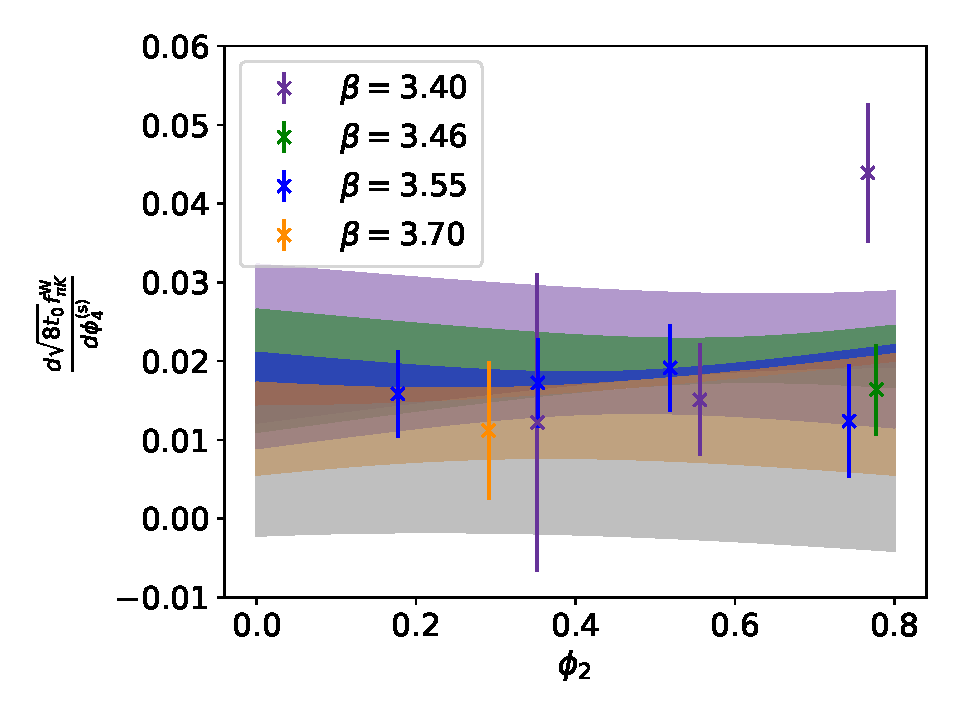
\includegraphics[width=1.\textwidth]{./cap4/figs/der_t0fpik.pdf}
    \caption{Derivative $d\left(\sqrt{8t_0}f_{\pi K}\right)/d\phi_4^{\textrm{(s)}}$ for the Wilson unitary setup. For the fit eq.~(\ref{ch_ma:eq:md_1}) was used. Results for the fit parameters are presented in Table~\ref{ch_ma:tab:md}.}
    \label{ch_ma:fig:dfpik_w}
\end{figure}

\begin{figure}
    \centering
    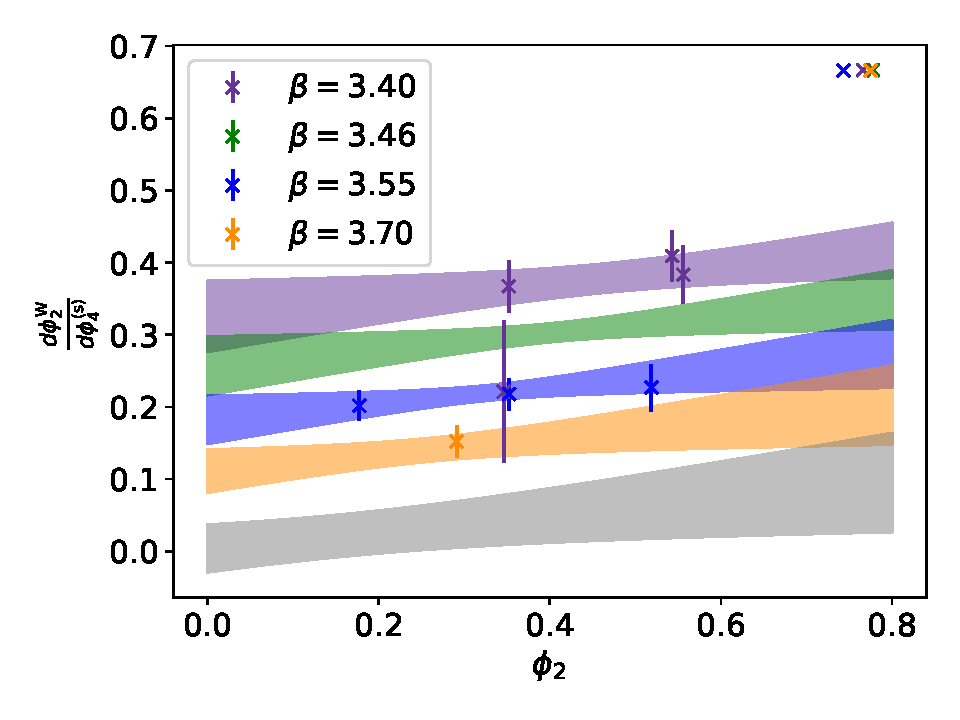
\includegraphics[width=1.\textwidth]{./cap4/figs/der_phi2.pdf}
    \caption{Derivative $d\phi_2/d\phi_4^{\textrm{(s)}}$ for the Wilson unitary setup. For the fit eq.~(\ref{ch_ma:eq:md_1}) was used. Results for the fit parameters are presented in Table~\ref{ch_ma:tab:md}. The points around $\phi_2\sim0.7$ correspond to the symmetric point at which by construction $\phi_2=\frac{2}{3}\phi_4$.}
    \label{ch_ma:fig:dphi2_w}
\end{figure}

\begin{figure}
    \centering
    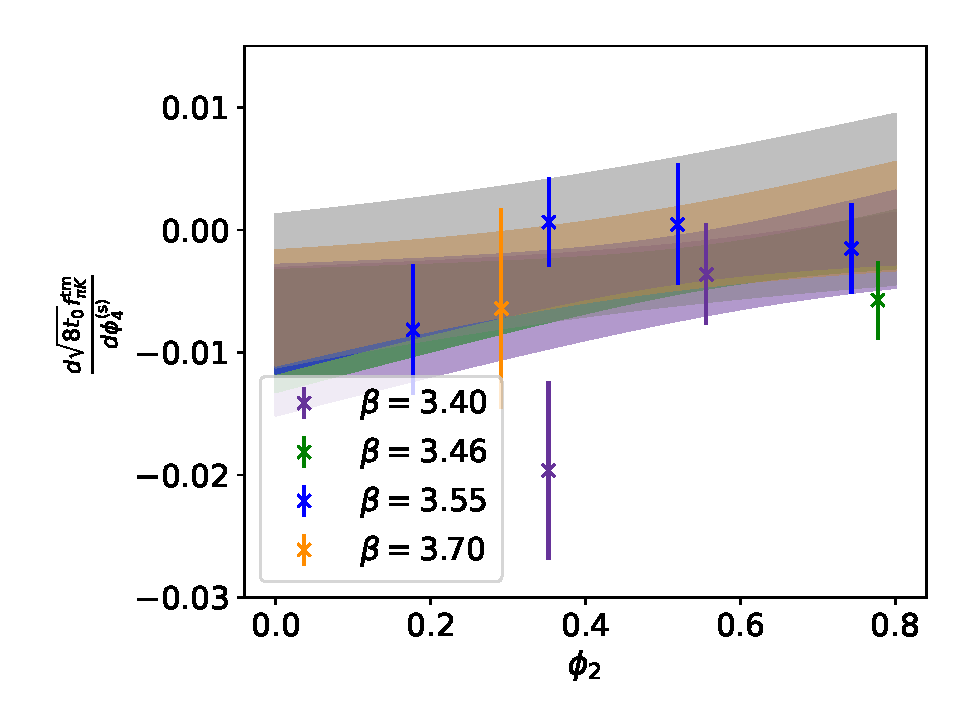
\includegraphics[width=1.\textwidth]{./cap4/figs/der_sea_t0fpik.pdf}
    \caption{Derivative $d\left(\sqrt{8t_0}f_{\pi K}\right)/d\phi_4^{\textrm{(s)}}$ for the mixed action setup. For the fit eq.~(\ref{ch_ma:eq:md_1}) was used. Results for the fit parameters are presented in Table~\ref{ch_ma:tab:md}.}
    \label{ch_ma:fig:dfpik_tm}
\end{figure}

\begin{figure}
    \centering
    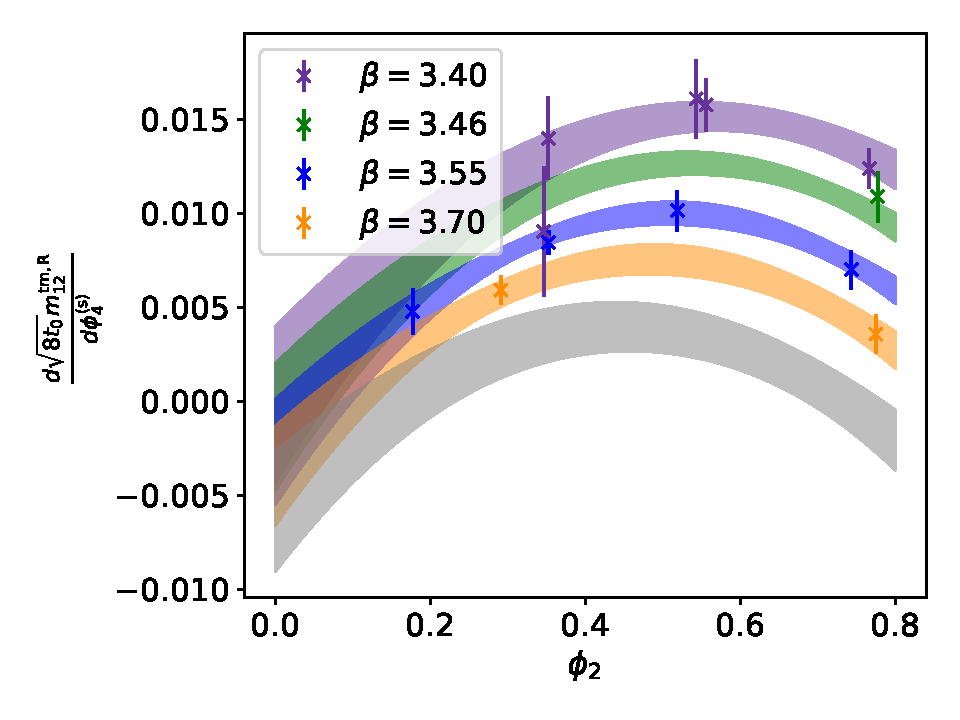
\includegraphics[width=1.\textwidth]{./cap4/figs/der_sea_t0m12.pdf}
    \caption{Derivative $d\left(\sqrt{8t_0}m_{12}^{\textrm{R}}\right)/d\phi_4^{\textrm{(s)}}$ for the mixed action setup. For the fit eq.~(\ref{ch_ma:eq:md_2}) was used. Results for the fit parameters are presented in Table~\ref{ch_ma:tab:md}.}
    \label{ch_ma:fig:dm12_tm}
\end{figure}

\begin{figure}
    \centering
    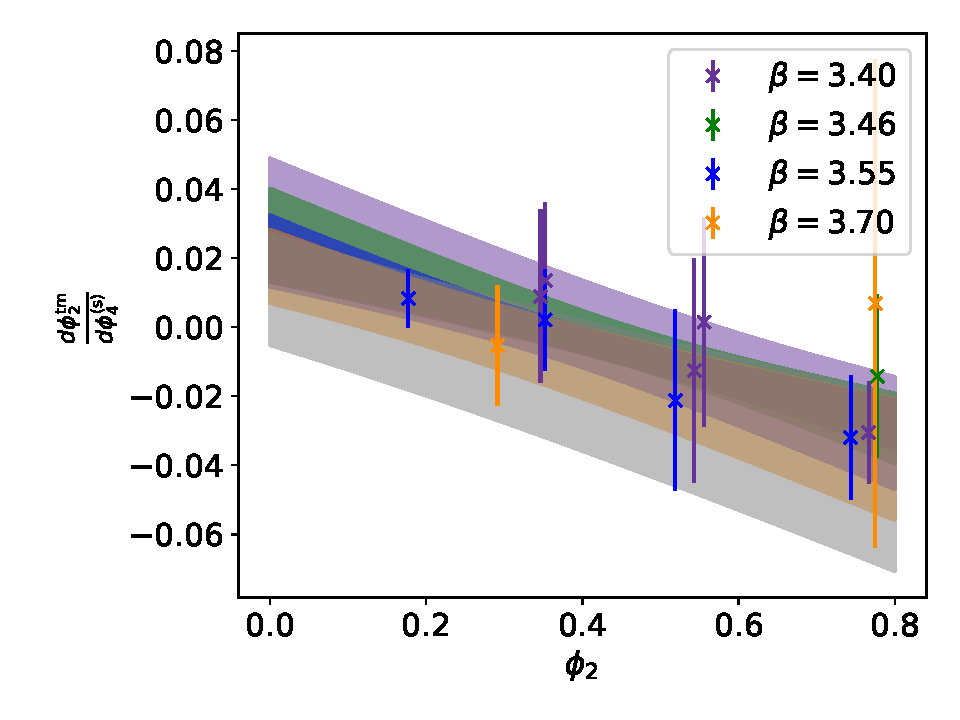
\includegraphics[width=1.\textwidth]{./cap4/figs/der_sea_phi2.pdf}
    \caption{Derivative $d\phi_2/d\phi_4^{\textrm{(s)}}$ for the mixed action setup. For the fit eq.~(\ref{ch_ma:eq:md_1}) was used. Results for the fit parameters are presented in Table~\ref{ch_ma:tab:md}.}
    \label{ch_ma:fig:dphi2_tm}
\end{figure}

\begin{figure}
    \centering
    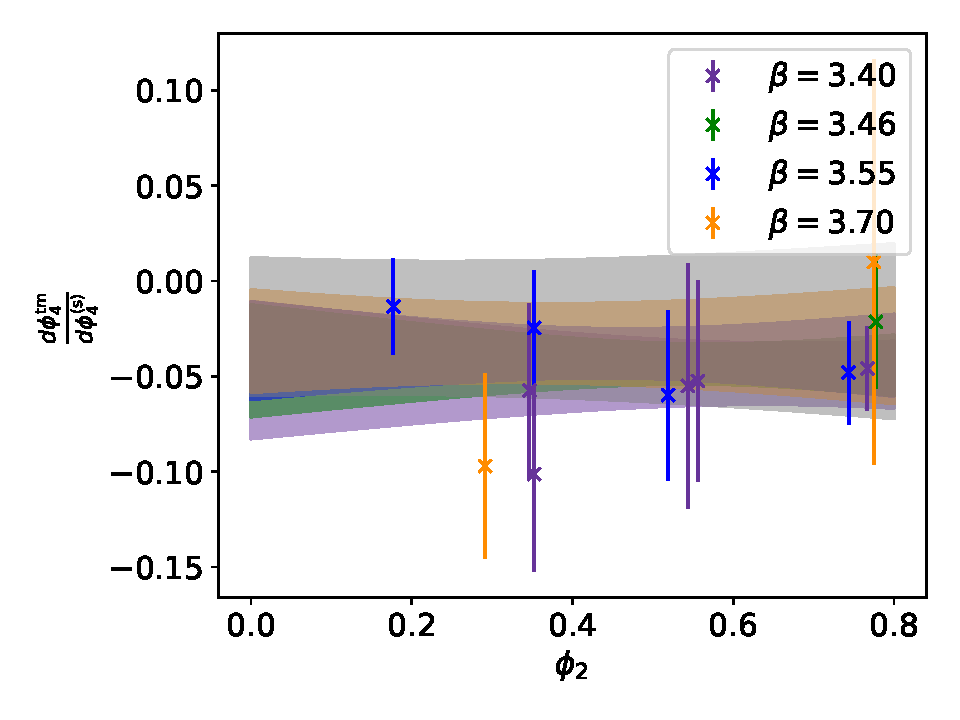
\includegraphics[width=1.\textwidth]{./cap4/figs/der_sea_phi4.pdf}
    \caption{Derivative $d\phi_4/d\phi_4^{\textrm{(s)}}$ for the mixed action setup. For the fit eq.~(\ref{ch_ma:eq:md_1}) was used. Results for the fit parameters are presented in Table~\ref{ch_ma:tab:md}.}
    \label{ch_ma:fig:dphi4_tm}
\end{figure}

%%%%%%%%%%%%%%%%%%%%%%%%%%%%%%%%%%%%%%%%%%%%%%%%%%%%%%%%%%%
%%%%%%%%%%%%%%%%%%%%%%%%%%%%%%%%%%%%%%%%%%%%%%%%%%%%%%%%%%%
%%%%%%%%%%%%%%%%%%%%%%%%%%%%%%%%%%%%%%%%%%%%%%%%%%%%%%%%%%%
%%%%%%%%%%%%%%%%%%%%%%%%%%%%%%%%%%%%%%%%%%%%%%%%%%%%%%%%%%%


\section{Matching and tuning to full twist}
\label{ch_ma:sec:matching}

As explained in Sec.~\ref{ch_ma:sec:Valence}, when working with a mixed action, after performing the mass shifts in Sec.~\ref{ch_ma:sec:chiral_traj}, we need to match the physical quark masses of the sea and valence sectors. To do this, we use a grid of valence parameter values to find the target point through small interpolations. For the values of the relevant observables in the sea sector, we employ measurements in the fully Wilson unitary setup. In practice, to compute the physical values (renormalized and improved) of quark masses we need the relevant improvement coefficients. In order not to rely on these for the matching procedure, instead of matching the physical quark masses we choose to use the pion and kaon masses in units of the gradient flow scale $t_0$
\begin{align}
\label{ch_ma:eq:matching}
\phi_2^{\textrm{(s)}}&=\phi_2^{\textrm{(v)}},\\
\phi_4^{\textrm{(s)}}&=\phi_4^{\textrm{(v)}}.
\end{align}
since these quantities are proportional to the renormalized quark masses at LO in ChPT (see eqs.~(\ref{ch_ma:eq:phi2}-\ref{ch_ma:eq:phi4})).

Furthermore, we need to tune the Wilson tm action to full twist, which means setting the valence light PCAC quark mass to zero
\begin{equation}
\label{ch_ma:eq:full-twist}
m_{ud}^{\textrm{(v)}}\equiv m_{ll'}^{\textrm{(v)}}\equiv m_{12}^{\textrm{(v)}}=0.
\end{equation}
Setting the maximal twist condition through a vanishing value of the light valence PCAC quark mass, as in eq~(\ref{ch_ma:eq:full-twist}), is sufficient to guarantee the absence of lattice artifacts of $\mathcal{O}(a)$ in physical observables~\citep{Frezzotti:2003ni, ETM:2008zte}. 

To impose eqs.~(\ref{ch_ma:eq:matching}-\ref{ch_ma:eq:full-twist}), we perform interpolations of the valence observables $m_{12}^{\textrm{(v)}},\phi_2^{\textrm{(v)}},\phi_4^{\textrm{(v)}}$ in the $\left(\kappa,\mu_l,\mu_s\right)^{\textrm{(v)}}$ hyperplane, using as fit functions the following expressions motivated by ChPT
\begin{align}
m_{12}^{\textrm{(v)}}&=p_1\left(\frac{1}{\kappa^{\textrm{(v)}}}-\frac{1}{\kappa^{\textrm{(v)*}}}\right)+p_2\left(\mu_l^{\textrm{(v)}}-\mu_l^{\textrm{(v)*}}\right),\\
\phi_2^{\textrm{(v)}}&=\frac{p_3}{\mu_l^{\textrm{(v)}}}\left(\frac{1}{\kappa^{\textrm{(v)}}}-\frac{1}{\kappa^{\textrm{(v)*}}}\right)^2+p_4\left(\mu_l^{\textrm{(v)}}-\mu_l^{\textrm{(v)*}}\right)+\phi_2^{\textrm{(s)}},\\
\phi_4^{\textrm{(v)}}&=\frac{p_5}{\mu_l^{\textrm{(v)}}}\left(\frac{1}{\kappa^{\textrm{(v)}}}-\frac{1}{\kappa^{\textrm{(v)*}}}\right)^2+\frac{p_6}{\mu_s^{\textrm{(v)}}}\left(\frac{1}{\kappa^{\textrm{(v)}}}-\frac{1}{\kappa^{\textrm{(v)*}}}\right)^2 \notag \\
&+p_7\left(\mu_l^{\textrm{(v)}}-\mu_l^{\textrm{(v)*}}\right)+p_8\left(\mu_s^{\textrm{(v)}}-\mu_s^{\textrm{(v)*}}\right)+\phi_4^{\textrm{(s)}}.
\end{align}
In this way, the target point values $\left(\kappa,\mu_l,\mu_s\right)^{\textrm{(v)*}}$ are found as fit parameters of a simultaneous fit of these three quantities. The interpolation is shown in Fig.~\ref{ch_ma:fig:match}.

The mixed action results for the quark masses are given by the target twist mass parameters $\mu_{l,s}^{\textrm{(v)*}}$, while the extraction of the pion and kaon decay constants in the mixed action setup requires an additional interpolation along the valence grid to the target point. The fit functions for this interpolation are
\begin{align}
f_{\pi}^{\textrm{(v)}}&=q_1\left(\frac{1}{\kappa^{\textrm{(v)}}}-\frac{1}{\kappa^{\textrm{(v)*}}}\right)^2+q_2\left(\frac{1}{\kappa^{\textrm{(v)}}}-\frac{1}{\kappa^{\textrm{(v)*}}}\right)+q_3\mu_l^{\textrm{(v)}},\\
f_K^{\textrm{(v)}}&=r_1\left(\frac{1}{\kappa^{\textrm{(v)}}}-\frac{1}{\kappa^{\textrm{(v)*}}}\right)^2+r_2\left(\frac{1}{\kappa^{\textrm{(v)}}}-\frac{1}{\kappa^{\textrm{(v)*}}}\right)+r_3\mu_l^{\textrm{(v)}}+r_4\mu_s^{\textrm{(v)}}.
\end{align}
The interpolation for the decay constants combination $f_{\pi K}$ defined in eq.~(\ref{ch_ss:eq:fpik}) is shown in Fig.~\ref{ch_ma:fig:fpik_interp}.

\begin{figure}
    \centering
    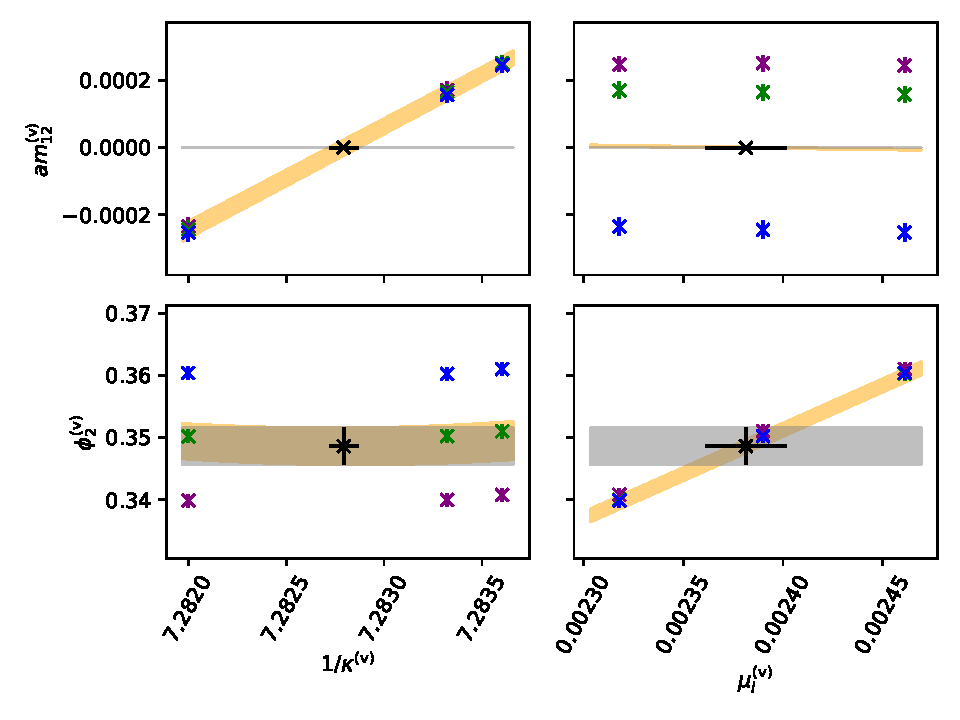
\includegraphics[width=1.\textwidth]{./cap4/figs/matching_N200.pdf}
    \caption{Matching of sea (gray horizontal band) and valence values of $\phi_2$ (lower panels) and tuning to full twist $am_{12}^{\textrm{(v)}}=0$ (upper panels) along the grid of valence parameters values for the ensemble N200. Each point represents a different measurement in the valence along the grid, and the orange band represents the interpolation. The black point is the target result $\left(\kappa,\mu_l,\mu_s\right)^{\textrm{(v)*}}$. Here we only show the matching of $\phi_2^{\textrm{(v)}}$ and $am_{12}^{\textrm{(v)}}$, though the matching of $\phi_4^{\textrm{(v)}}$ is done simultaneously.}
    \label{ch_ma:fig:match}
\end{figure}

\begin{figure}
    \centering
    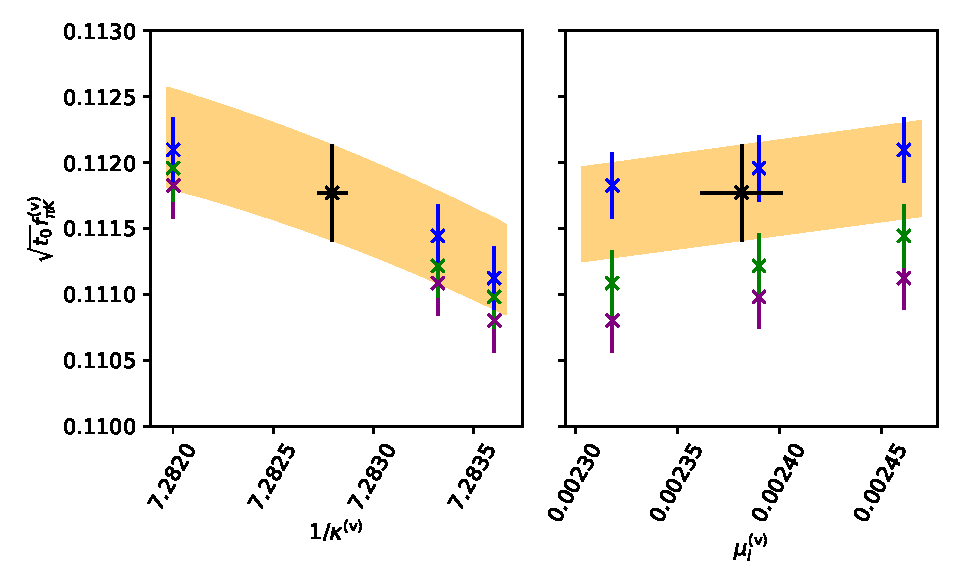
\includegraphics[width=1.\textwidth]{./cap4/figs/interp_fpik_N200.pdf}
    \caption{Interpolation of $\sqrt{t_0}f_{\pi K}$ (see eq.~(\ref{ch_ss:eq:fpik})) along the valence grid to the target point $\left(\kappa,\mu_l,\mu_s\right)^{\textrm{(v)*}}$ for the ensemble N200. The points with different colors represent measurements at different values of the valence parameters.}
    \label{ch_ma:fig:fpik_interp}
\end{figure}

%%%%%%%%%%%%%%%%%%%%%%%%%%%%%%%%%%%%%%%%%%%%%%%%%%%%%%%%%%%
%%%%%%%%%%%%%%%%%%%%%%%%%%%%%%%%%%%%%%%%%%%%%%%%%%%%%%%%%%%
%%%%%%%%%%%%%%%%%%%%%%%%%%%%%%%%%%%%%%%%%%%%%%%%%%%%%%%%%%%
%%%%%%%%%%%%%%%%%%%%%%%%%%%%%%%%%%%%%%%%%%%%%%%%%%%%%%%%%%%
